\documentclass[12pt,openright,a4paper]{article}
\setlength{\parindent}{1.3cm}
\setlength{\parskip}{0.2cm}
\usepackage[alf]{abntex2cite}
\usepackage{graphicx}
\usepackage{indentfirst} 
\usepackage{lmodern}
\usepackage{listings}
\pagenumbering{arabic}
\usepackage{lineno}
\usepackage{float}
\usepackage{amsmath}
\linenumbers




\begin{document}
	\linespread{1.5}
 \fontsize{16}{10}\selectfont \centering \textbf{Analysis of computer science newcomers student's motivation} \\
	\fontsize{14}{10}\selectfont {Analysis of student's motivation}\newline

\fontsize{12}{10}
\flushleft
	\textbf{Authors:}\\
	\textbf{Student name:} Felipe Augusto Ferreira de Castro\\
	\textbf{Affiliations:} Federal University of Uberlandia\\
	\textbf{Email:} felipeaugusto.ferreiradecastro@gmail.com \newline
	
\textbf{Professor name:} João Henrique de Souza Pereira\\
\textbf{affiliations:} Federal University of Uberlandia\\
\textbf{email:} joaohs@ufu.br\newline

\textbf{Number of pages:19}\\
\textbf{Number of figures:11}\\
\textbf{Number of tables:0}\\
\textbf{Abstract word number:132}\\
\textbf{introdution word number:304}\\
\textbf{discussion word number:417}\newline
	
\textbf{Acknowledgments}\\	
My thanks to comppet group that lent me a room to make all data collecting and to all 4 volunteers who made the project possible.\newline

\textbf{conflicts of interest}\footnote{The authors declare no competing financial interests.}

\newpage
\tableofcontents
\newpage
\section{Abstract}
Depression and other mind diseases are currently being reported at universities. Due to it, this research was proposed to observe a group of newcomers students of the Federal University of Uberlandia (UFU) along two semesters. Furthermore, resources provided by BCI (Brain computer interface)  technology were used to collect an amount of data about their emotional state.

Data collecting were made on 3 points of semester and each one was proposed to the volunteers to do  same activity related to computer science course. They executed those activities  while wearing a EEG based equipment, Epoc+, which was responsible for collecting their emotional data.
The results were satisfying,  students became more stressed along time and their excitement decreased.     Surprisingly relaxation has increased, different from what was expected. The other feelings had no great changes, though.

The results were satisfying,  students became more stressed along time and their excitement decreased.     Surprisingly relaxation has increased, different from what was expected. The other feelings had no great changes, though.
\section{Significance Statement}
Mental diseases such as depression, stress, anxiety and other, had increased in our society nowadays.  According to World health organization (WHO)  more than 300 million people of all ages suffer from the disease, furthermore, as cited in G1 between 2005 and 2015 in Brazil anxiety cases increased 14,9\% and the country is the first one in related cases of the illness on Latin America, with 5,8\% of the population affected. 

The researcher Michelle Guimarães believes that detecting mental disorders can be a indicator of mental healthiness on young students and also she defends that those diseases reduces students productiveness. Due to it, this paper intend to detect the mental mood of students using Brain computer interface and appraise changes along time.  
\section{Introduction}
Due to the recent increase of mental illness cases in universities, such as depression, anxiety and other. This paper main goal is to get a emotional mood change of newcomers university students along the first two semester of their course. The course analyzed was computer science in Federal University of Uberlandia and the data collecting was done while the volunteers were doing same activities related to the course, for example programming and mathematics exercises.

A brain activity detection can be done by two kind of methods, invasive and non-invasive. The invasive  are base in physical implants of electrodes for brain waves detection, a non- invasive involves using, for example, Magnetic resonance or Electroencephalogram (EEG) to measure brain activities. This methods detect different waves types, such as, Gamma in frequency range of 31Hz  an up, Beta waves in range of 12 and 30 Hz, Alpha waves ranging from 7.5 to 12 Hz , Theta waves from 3.5 to 7.5Hz and Delta waves frequency from 0.5 to 3.5 Hz. The Beta and Gamma waves are related to cognition activities and perception, the Alpha is associated to relaxation and disengagement, Theta wave is related to stress, frustration and in the end Delta waves are related to physical defects in the brain (Larsen, 2011).

Researches about identifying emotion based on EEG, technology used on this paper, are relatively  new and many researchers use beta and alpha waves to do it (Matlovic, 2016). The equipment used was Emotiv EPOC+,  which is EEG based and has support to same emotional states detection, those are stress, Focus, engagement, Relaxation, Interest and Excitement, the software used were Emotiv Xavier control panel (Emotiv Github, 2019) and the EmotivBCI (Emotiv, 2019). Both makes possible to calibrate the device to each student and build a percentage result of it emotion through time.
\section{Materials and Methods}

\subsection{Materials}

The material used was Epoc+ of Emotiv, that can take waves from 0.16 Hz until 43 Hz(Comparison chart, 2019). As well, some codes in c language were used during tests.

\subsection{Method}
 \subsubsection{Study object}
 The group of volunteers was taken from the newcomers class of 2018-2º semester of Federal University of Uberlandia Computation Faculty.  Due to the difficult of building a probability sample in a class with around 60 students, it was opted for a not probability sample. Although, it would not affect the results of the research, because not probability sample many times have similar results with probability samples (Manzato, 2012). The 4 students were choosen randomly, being 3 men and 1 woman.
 \subsubsection{Proposed Activities}
 During 2 semesters 5 data collects were made, around 15 minutes each, 2 on the first semester and 3  on the second semester, it happened because of a problem with internet during the second data collect of the first semester. The activities proposed were :
 
 \begin{enumerate}
 	\item The data was collected using the Software Xavier Control panel 3.5.1 and annotated handily on Microsoft excel tables.
 	 the proposed activity was a semi-structured interview with the following questions:\newline
 	 Question 1 - Describe how was your experience and hopes after enter the first time in the university. Some of that hopes were fulfilled ? \newline
 	 Question 2  - There a lot differences between academic life before and after entering a university. Can you cite some of them that happened to you? Which of them affected you the most ?\newline
 	 Question 3 – How your relationship with the professors is?\newline
 	 Question 4 – Many times university is the begin of adult life adding some new responsibilities. Did you have any new responsibilities after entering university ? How do you deal with them ?\newline
 	 
 	 Each of these question were made with a goal :\newline
 	 1- Try to persuade the student to feel as he did with his first experiences at university;\newline
 	 2-  To influence the volunteer to ponder about how his life has changed and if those changes were good or bad;\newline
 	 3 and 4 – The main goal of it is to persuade the student to think about his new life at university, new relationships and how they felt about it.\newline
  \item  The Second data collect was not concluded.
  \item That data collect was made using 2 software, Xavier control panel 3.5.1 and EmotivBCI, Both are free distributed by Emotiv. The proposed activity was programming in c language, which is contemplated by first semester grade of the course. A program c was given to them, that program had a syntax problem and they should correct it. 
  
  \item This collect was made on the second semester of the research. It, also, was a semi-structured interview with the following questions:\newline
  Question 1- Describe how was the experience in the previous semester.\newline
  Question 2 – How did you feel returning to university after vacation ? This feeling can on some way influence your future choices ?\newline
  Question 3 – How your relationship with professors is ? Compare with the professors on the previous semester. How do you deal with bad professors ?\newline
  
  Each of these questions were made with a goal:
  
  1 – Try to persuade the student to think about his experience on the previous semester;\newline
  2 – To influence the student to ponder about how his previous experiences affected his will to study and continue coming to college;\newline
  3 -  The main goal is to persuade the student to think about how his behavior with professors has changed or not.\newline
  
  \item The proposed activity was a integral calculus one, They had 15 minutes to solve the following:\newline
  
  		a- \[ \int\dfrac{dx}{\sin^2{3x - 1}} \]\newline
  		b- \[ \int (x^2 + 2x)e^x dx \]
  		
  		c- \[ \int \dfrac{\sqrt{a^2 - x^2}}{x^2}dx \]
  		
   \item The proposed activity was equal to the 5, only different functions were proposed:\newline
        a - \[ \int (\csc x  \cot x) dx  \] 
        b- \[ \int_{1}^{2} x \ln x dx \]
  It is important to notice that integral calculus is taught on first semester and they were on their second.
 \end{enumerate}
  \subsubsection{About semi-structured interview}
 The semi-structured interviews combine open and closed-ended questions, which the interviewed is able to develop and talk about the proposed theme. The interviewer must follow a set of pre determined questions, however it should be done on a enviroment similar to a informal conversation. The main advantage of open interviews and semi-strutured interviews is that both quite ever produce the better samples.
 
 Semi-structed interviews make possible a proximity between interviewed and interviewer, what  allows to the interviewer ask about more delicated issues, as well. That means, how less strutured the interview is, better the exchange will be between both participants (Boni, Quaresma, 2005).
 
 \subsection{Statistical Analyses}
 The software Xavier control panel and EmotivBCI, both, build a percentage result of each emotion through time. Based on that results the statistical analysis were built after each data collecting and after the end of them all.
 
 Microsoft Excel was used to build tables and graphics shown in this paper, as well the calculus of average and standard deviance. The analysis were all based on how high the standard deviance was between students and through time. There are not any other complex calculus in the paper.  
 \newpage
\section{Results}
 The research has shown satisfactory results. As well as expected, the students stress increased and excitement values of volunteers N1 and N2  reduced along time. The student N3 showed to be a outlier, due to it, the results will be divided by calculus counting with N3 and not counting with it.
 
 Observing each emotion individually it’s possible to realize that:
 \begin{itemize}
 	\item Stress: It’s one of the most important emotions on this paper and it has shown expected results. Furthermore, its values raised constantly along data collecting with a standard deviation around 33\% including student N3 and 23\% without N3 values.
 	  \begin{figure}[H]
 	  	\centering
 	  	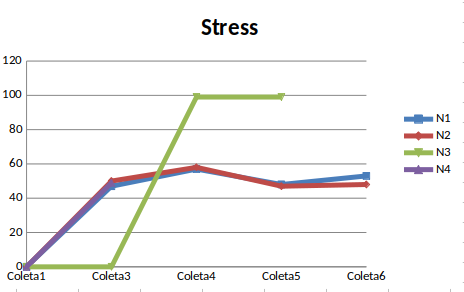
\includegraphics[width=10cm]{./stress.png}
 	  	\caption{students stress values along data collecting}
 	  \end{figure}
 	\item Focus: The Behavior of Focus was different on each participant, it presented low values variance from the beginning of the research until its end, as it is able to be concluded by standard deviation of 11\%. 
 	   \begin{figure}[H]
 	  	\centering
 	  	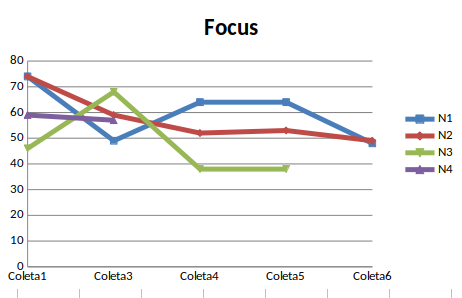
\includegraphics[width=10cm]{./focus.png}
 	  	\caption{students focus values along data collecting}
 	  \end{figure}
 	\item Relaxation: Another important emotion to this paper, which has shown controversial feedback, due to constant rise of values along data collecting. The emotion has not shown high differences between students, hence standard deviation of it was approximately 7\% without student N3 and around 14\% within N3.
 	  \begin{figure}[H]
 	 	\centering
 	 	\includegraphics[width=10cm]{./relaxation.png}
 	 	\caption{students relaxation values along data collecting}
 	 \end{figure}
 	\item Interest: Interest behavior was quite the same through all data collects. The values of it had little variances and the lowest standard deviation of all emotions, under 7\% even considering N3 in calculus. 
 	     \begin{figure}[H]
 	    	\centering
 	    	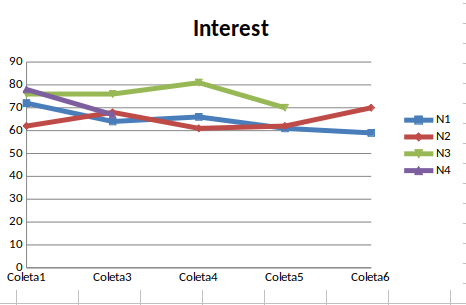
\includegraphics[width=10cm]{./interest.png}
 	    	\caption{students interest values along data collecting}
 	    \end{figure}
 	\item Excitement: This feeling presented high alterations on student N3, a big increase from first data collect to last one, it has shown same lower values in mid term collects though. The standard deviation values was around 14\% considering participant N3 and 12\% without him.
 	      \begin{figure}[H]
 	     	\centering
 	     	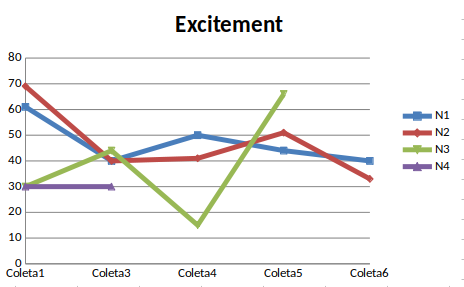
\includegraphics[width=10cm]{./excitement.png}
 	     	\caption{students exitement values along data collecting}
 	     \end{figure}
 	\item Engagement: Students N2 and N4 presented a high difference from collect 1 to 3, that increase was around 56\%. while that, students N1 and N3 did not show significant changes in them values. The general Standard deviation was 21\%, however building groups of students with N1 and N2 being first group and N2 and N4 a second, it makes possible to notice that N1 and N3 had no big changes, since standard deviation of the group was 6\%. It is not possible to say same of N2 and N4, because their standard deviation was around 30\%.       
 	    \begin{figure}[H]
 	   	\centering
 	   	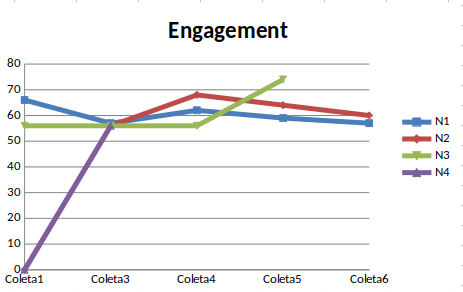
\includegraphics[width=10cm]{./engagement.png}
 	   	\caption{students engagement values along data collecting}
 	   \end{figure}
 \end{itemize}
\newpage
\section{Discussion}
\subsection{About the emotions on the paper}
In order to a better understanding of any emotion on this paper follows the meaning of each according to Cambridge University dictionary:
\begin{itemize}
	\item Relaxation: Feeling that makes who feel it more calm, less worried;
	\item Engagement: Disposition to do something;
	\item Excitement: Feeling of being excited;
	\item Interest: The wish of pay attention on something, to discover more about it;
	\item Stress: Huge worry about a situation or something that may cause it;
	\item Focus: Pay attention to a particular activity.
\end{itemize}

\subsection{About Results}
Along time it is possible to realize a increase in students values of Relaxation and stress. Excitement, Focus, Interest showed a decrease and Engagement the lowest changes on the same student. It is possible to see the values change by the collecting graphics :
\begin{itemize}
\item Collect 1 : Only one made with all four volunteers.
\begin{figure}[H]
	\centering
	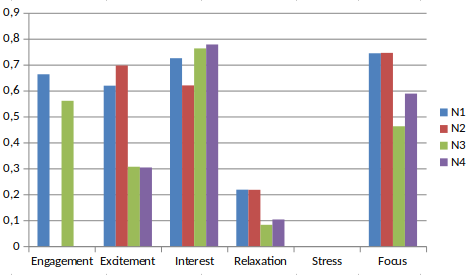
\includegraphics[width=10cm]{./Coleta1.png}
    \caption{Coleta 1 results}
\end{figure}
\item Collect 2: That Collect data was lost due to a internet problem during the test.

\item Collect 3: participants N1, N2 and N3.
\begin{figure}[H]
	\centering
	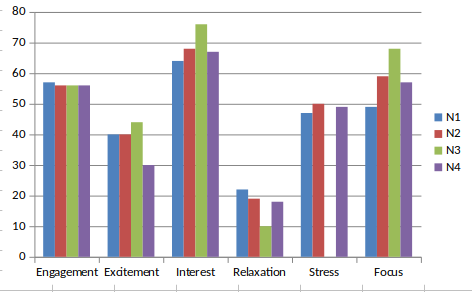
\includegraphics[width=10cm]{./Coleta3.png}
	\caption{Coleta 3 results}
\end{figure}
\item Collect 4: participants N1, N2 and N3.
\begin{figure}[H]
	\centering
	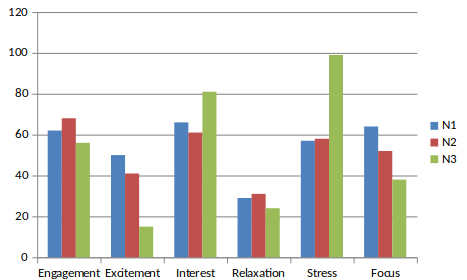
\includegraphics[width=10cm]{./Coleta4.png}
	\caption{Coleta 4 results}
\end{figure}
\item Collect 5 : participants N1, N2 and N3..
\begin{figure}[H]
	\centering
	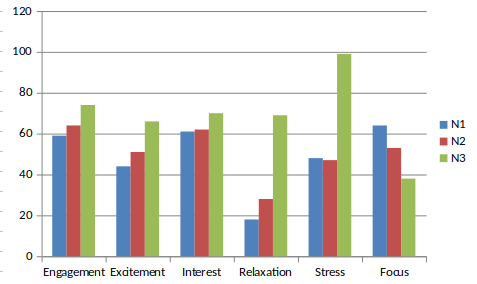
\includegraphics[width=10cm]{./Coleta5.png}
	\caption{Coleta 5 results}
\end{figure}
\item Collect 6: Due to same personal problems student N3 did not participated in this data collecting. Participants N1 and N2.  
\begin{figure}[H]
	\centering
	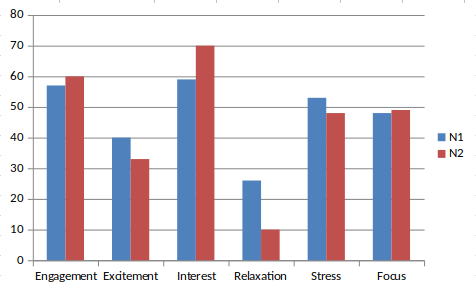
\includegraphics[width=10cm]{./Coleta6.png}
	\caption{Coleta 6 results}
\end{figure}

\end{itemize}


\subsection{validation}
The used equipment Epoc+ from Emotiv is able to detect waves of frequecy from 0.16 Hz until 43 Hz(Comparison chart, 2019), that means it can capture from Delta waves up to Gamma waves. Furthermore, according to some researchers Beta and Alpha waves are enough to emotion detection (Matlovic, 2016).  

Relaxation and Stress have, both, increase and it may be controversial, due to their contrary nature. Although, a possible interpretation to that fact is that students would be more used to university environment and all differences in their lives before and after college, what could has made them more comfortable, what would explain the relaxation increase. As well, the stress increase could be explained  by the university mood, which in Brazil, is highly different from high school mood.
\newpage
\subsection{Significance of this work}
In Brazil around 30\% of population economically active has already get some level of stress, due to excessive pressure (Santos, Maia, Faeda, Gomes, Nunes, Oliveira, 2017). Furthermore, in universities that reality is not different. Hence, what this paper propose is to use new technologies, like BCI, to try identify mental disorders and, perhaps, use it to number how intense the problem is in order to do create a tool to be used by mental illness professionals, as psychologists and psychoanalysts.

\newpage
\section{References}

  Antonio J. Manzato (2012) A Elaboraçao de questionários na pesquisa quantitativa (Portuguese).Source: http://www.inf.ufsc.br/~vera.carmo/Ensino\_2012\_1/ELABORACAO\\ \_QUESTIONARIOS \_PESQUISA\_QUANTITATIVA.pdf\newline
   
  Dictionary Cambridge (2019) Relaxation. Source: https://dictionary.cambridge.org/dictionary/english/relaxation\newline
  
  Dictionary Cambridge (2019) Engagement. Source: https://dictionary.cambridge.org/dictionary/english/engagement\newline
   
  Dictionary Cambridge (2019) Excitement. Source: https://dictionary.cambridge.org/dictionary/english/excitement\newline
   
  Dictionary Cambridge (2019) Interest. Source: https://dictionary.cambridge.org/dictionary/english/interest\newline
  
  Dictionary Cambridge (2019) Stress. Source: https://dictionary.cambridge.org/dictionary/english/stress\newline
  
  Dictionary Cambridge (2019) Focus. Source: https://dictionary.cambridge.org/dictionary/english/focus\newline
  
  Emotiv (2019) EmotivBCI. Source: https://www.emotiv.com/emotiv-bci/ \newline
  
  Emotiv Comparison Chart (2019) Headset Comparison Chart. Source: https://www.emotiv.com/comparison/ \newline
  
  Emotiv GitHub (2019) Emotiv Software Development kit. Source: https://github.com/Emotiv/community-sdk/tree/master/tools \newline
  
  Erik A. Larsen (2011) Classification of EEG Signals in a Brain-Computer Interface System. Source: https://ntnuopen.ntnu.no/ntnu-xmlui/handle/11250/252472 \newline
  
  Fernando S. Santos, Carlos R. C. Maia, Fernanda C. Faedo, Melriden E. Nunes, Marcos V. M. de Oliveira (2017) Stress among Pre-University and Undergraduate
  Medical Students. Source: http://www.scielo.br/pdf/rbem/v41n2/1981-5271-rbem-41-2-0194.pdf \newline
  
  G1 (2017) Depressão cresce no mundo, segundo OMS; Brasil tem maior prevalência da América Latina (Portuguese). Source:https://g1.globo.com/bemestar/noticia/depressao-cresce-no-mundo-segundo-oms-brasil-tem-maior-prevalencia-da-america-latina.ghtml.\newline
  
  Michelle Guimarães (2014) Depressão,Ansiedade,Estresse e Qualidade de vida dos estudantes de universidade pública e privada (Portuguese).Source: http://tede.metodista.br/jspui/handle/tede/1348 \newline 
  
  Thomas Mastlovic (2016) Emotion Detection using EPOC EEG device. Souce: https://pdfs.semanticscholar.org/c8e5/a8315ada36be049a\\74232f561b64ab9bb120.pdf \newline
  
  Valdete Boni, Sílvia J. Quaresma (2005) Aprendendo a entrevistar: como fazer entrevistas em Ciências Sociais (Portuguese).Revista Eletrônica dos Pós-graduandos em Sociologia Política da UFSC 2:68-80.\newline
  
  World Health Organization(2018) Depression. Source: https://www.who.int/en/news-room/fact-sheets/detail/depression \newline
  
  
\end{document}